\section{System agentowy}
%%%% OPIS NARZĘDZI - plusy i minusy
Na rys. \ref{fig:actor} został umieszczony schemat stworzonej przez zespół architektury systemu agentowego.
\begin{figure}[!htb]
\centering
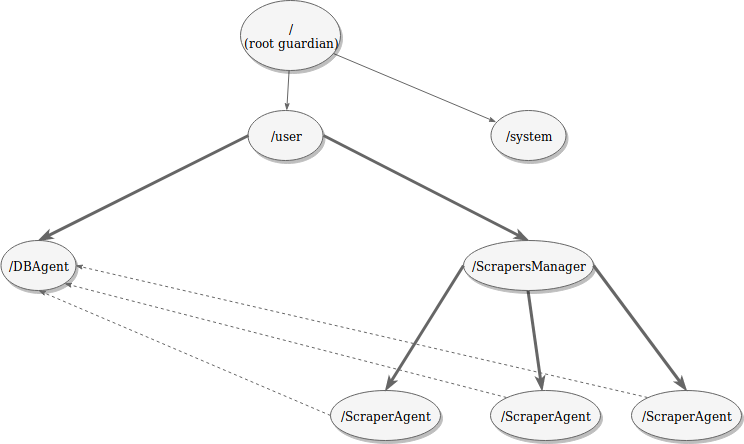
\includegraphics[width=1.0\textwidth]{./pict/actors.png}
\caption{Schemat wdrożonego systemu zgodnie z architekturą Akka}
\label{fig:actor}
\end{figure}

\par Przy czym strzałki pogrubione oznaczają podległość agentów (aktorzy przy końcu strzałki są ''dziećmi'' aktorów z początku strzałki), natomiast dodatkowe strzałki przerywane oznaczają kierunek wysyłania wiadomości do agentów.

\par Poszczególni agenci w systemie różnią się między sobą zadaniami:
\begin{itemize}
	\item \texttt{DBAgent} - pełni zadania agenta mającego bezpośredni dostęp do bazy danych, w której składowane są artykuły. 
\end{itemize}

\par System ten został wykorzystany z użyciem popularnego dla takich celów frameworku Akka oraz języka Scala.

W stworzonym przez zespół systemie część agentów może działać w innych węzłach niż pozostałe. Dzięki wykorzystaniu biblioteki \texttt{Akka Remoting}, zespół przetestował umieszczenie osobno agenta ScrapersManager oraz wszystkich agentów typu ScraperAgent.

\subsection{Język Scala}

\subsection{Framework Akka}

\subsection{Schemat pobierania wiadomości}

Agenty odpowiedzialne za pobieranie oraz parsowanie artykułów, uruchamiane są 
regularnie.
Do pobierania danych z kanału RSS wykorzystano bibliotekę 
\texttt{ROME}, która dla zadanego adresu url pobiera tak zwany \texttt{feed}. Następnie za pomocą narzędzia \texttt{jsoup} 
pobierane oraz parsowane są treści każdego artykułu. 
Następnie treść każdego artykułu poddawany jest wektoryzacji w module NLP. W kolejnym kroku najważniejsze informacje o artykule:
\begin{itemize}
\item adres strony z której został pobrany,
\item strona z której został pobrany,
\item text artykułu,
\item data publikacji,
\item tagi,
\item oraz wektor zwrócony przez moduł NLP,
\end{itemize}
są zapisywane w bazie danych (rys. \ref{fig:db}).

\begin{figure}[ht!]
\centering
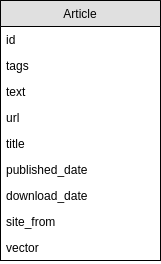
\includegraphics[height=0.3\textheight, width=0.3\textwidth]{./pict/db.png}
\caption{Schemat bazy danych}
\label{fig:db}
\end{figure}